\documentclass[a4paper]{article} %四号=14pt,小四=12pt,五号=10.5pt
\usepackage[heading=true]{ctex} %设置中文章节标题
\usepackage{graphicx} %插图
\usepackage{float} % 使用H控制浮动
\usepackage[section]{placeins} %限制浮动范围
\usepackage{booktabs} %使用三线表
\usepackage{listings} %使用环境lstlisting
\usepackage{minted} %使用环境minted排程序更美观,需要python包Pygments
\usepackage{xcolor} %使用color
\usepackage{enumerate}
\usepackage{amsmath}
\usepackage{amssymb} %mathbb
\usepackage{amsthm} %proof
\usepackage{geometry} %调整页边距与word相同
%margin=1in
\usepackage{algorithm}
% \usepackage{algorithmicx}
\usepackage{algpseudocode}
\usepackage[colorlinks=true]{hyperref} %超链接,为减少冲突,需要将其放在其他宏包之后。
\numberwithin{equation}{section} %按节编号
% \setcounter{tocdepth}{3}

\newcommand{\degree}{^\circ}
\newcommand{\ud}{\,\mathrm{d}}

\newtheorem{Theorem}{定理}

\title{\heiti 不等式选讲}
\author{\kaishu 余周炜\thanks{Email: \href{mailto:yuzhouwei6326@outlook.com}{yuzhouwei6326@outlook.com}}}
\date{\today}
\begin{document}
% \frontmatter
\maketitle


\clearpage
\tableofcontents

% \mainmatter
\newpage
\section{均值不等式}

设$a_1,a_2,\cdots,a_n\in\mathbb{R^+}$,将

$$
A_n= \frac{a_1+a_2+\cdots+a_n}{n}=\frac{\sum_{i=1}^{n}a_i}{n} 
$$
$$
G_n= \sqrt[n]{a_1a_2\cdots a_n}=\left(\prod_{i=1}^n a_i\right)^{\frac{1}{n}}=\exp\left[\frac{1}{n}\sum_{i=1}^n\ln a_i\right]
$$
$$
H_n= \frac{n}{\frac{1}{a_1}+\frac{1}{a_2}+\cdots+\frac{1}{a_n}}=\frac{n}{\sum_{i=1}^{n}\frac{1}{a_i}}
$$
$$
Q_n= \sqrt{\frac{a_1^2+a_2^2+\cdots+a_n^2}{n}}=\sqrt{\frac{\sum_{i=1}^n a_i^2}{n}}
$$

分别叫做这n个正数的算术平均数、几何平均数、调和平均数和平方平均数,有下面的\textbf{均值不等式}成立:
\begin{equation}
H_n\le G_n \le A_n \le Q_n
\end{equation}

当且仅当$a_1=a_2=\cdots=a_n$时取等号。

\subsection{证明}

\begin{proof}
\begin{enumerate}
\item 当$n=1$时,显然成立。
\item 设$n=k(k\ge 1)$时,$A_k\ge G_k$,
$$
\underbrace{x_{k+1}+(k-1)G_{k+1}}_{k\quad  numbers}\ge k \sqrt[k]{x_{k+1}G_{k+1}^{k-1}}
$$
\item $n=k+1$时,
\begin{align*}
 &\frac{x_1+x_2+\cdots+x_k+x_{k+1}+(k-1)G_{k+1}}{k} \\
 &\ge G_k+\sqrt[k]{x_{k+1}G_{k+1}^{k-1}}  \\
& \ge 2\sqrt[2k]{G_{k}^{k}x_{k+1}G_{k+1}^{k-1}}=2G_{k+1}
\end{align*} 
\begin{align*}
\therefore (k+1)A_{k+1} &=x_1+x_2+\cdots+x_k+x_{k+1} \\
& \ge 2kG_{k+1}-(k-1)G_{k+1} \\
& =(k+1)G_{k+1} \implies A_{k+1}\ge G_{k+1}
\end{align*}
也成立。
\end{enumerate}

$\therefore \forall n\in\mathbb{N^+} ,A_n\ge G_n$
\end{proof}

\subsection{推广}

\subsubsection{加权算术-几何平均不等式}

不仅“均匀”的算术平均数和几何平均数之间有不等式,加权的算术平均数和几何平均数之间也有不等式。设$x_1,\cdots,x_n$和$p_1,\cdots,p_n$为正实数,并且$p_1+p_2+\cdots+p_n=1$,那么:
\begin{equation*}
p_1x_1+p_2x_2+\cdots+p_nx_n\ge x_1^{p_1}x_2^{p_2}\cdots x_n^{p_n}
\end{equation*}

\subsubsection{矩阵形式}

算术-几何平均不等式可以看成是一位向量系数的平均数不等式。对于二维矩阵,一样有类似的不等式:对于系数都是正实数的矩阵
\begin{equation*}
\begin{bmatrix}
a_{11}      & \cdots & a_{1k}      \\
\vdots & \ddots & \vdots \\ 
a_{n1}      & \cdots & a_{nk}
\end{bmatrix}
\end{equation*}

设
$$
A_{j} = \frac{1}{n} \sum_{i=1}^n a_{ij},\quad G_{i}=\sqrt[k]{\prod_{j=1}^k a_{ij}} 
$$,那么有:
$$
\sqrt[k]{A_1 A_2 \cdots A_k} \leqslant \frac{G_1 + G_2 + \cdots + G_n}{n}
$$

也就是说:对 k 个纵列取算术平均数,它们的几何平均小于等于对 n 个横行取几何平均数的算术平均。

\subsubsection{极限形式}

也称为\textbf{积分形式}:对任意在区间$[0,1]$上可积的正值函数$f$,都有:
\begin{equation}
\int_0^1 f(x)\ud x \ge \exp(\int_{0}^{1}\ln f(x)\ud x)
\end{equation}

这实际上是在算术-几何平均值不等式取成
$$ \frac {x_{1}+x_{2}+\cdots +x_{n}}{n}  \ge \exp ( \frac{\ln {x_1} + \ln {x_2} + \cdots + \ln {x_n}}{n} )
$$

后,将两边的黎曼和中的$n$趋于无穷大后得到的形式。

\section{幂平均不等式}

\textbf{幂平均}(power mean),也叫广义平均(generalized mean),是毕达哥拉斯平均(包含了算术,几何,调和平均)的一种抽象化。

若$p$是一非零实数,可定义实数$x_1,\cdots,x_n$的p次幂平均为
\begin{equation}
M_p(x_1,\cdots,x_n)=\left(\frac{1}{n}\cdot\sum_{i=1}^n x_i^p\right )^{\frac{1}{p}} 
\end{equation}

一般地,如果$p<q$,则$M_p(x_1,\cdots,x_n)\le M_q(x_1,\cdots,x_n)$ 且这两个平均相等当且仅当$x_1=x_2=\cdots=x_n$。 这由事实
\begin{equation}
\forall p\in\mathbb{R}, \frac{\partial M_p(x_1,\cdots,x_n)}{\partial p}\ge 0
\end{equation}

得出,上述不等式可由琴生不等式证明。

特别地,对$p\in\{-1,0,1,2\}$,幂平均不等式蕴含了均值不等式。

\begin{figure}[htbp]
\centering
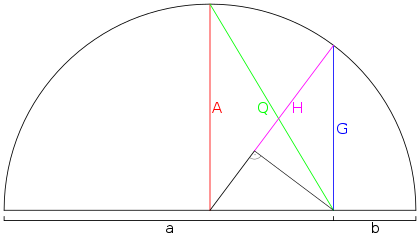
\includegraphics[width=0.5\textwidth]{mean.png}
\caption{特例:n=2时的图形描述}
\end{figure}

\subsection{特例}
最小值:
$$
M_{-\infty}(x_{1},\dots,x_{n})=\lim_{p\to -\infty }M_{p}(x_{1},\dots ,x_{n})=\min\{x_{1},\dots ,x_{n}\}
$$	
调和平均:
$$ 
M_{-1}(x_{1},\dots ,x_{n})=\frac{n}{\frac{1}{x_{1}}+\dots +\frac{1}{x_{n}}}
$$
几何平均:
$$
M_{0}(x_{1},\dots ,x_{n})=\lim_{p\to 0}M_{p}(x_{1},\dots ,x_{n})=\sqrt[n]{x_{1}\cdot \dots \cdot x_{n}}	
$$
算术平均
$$
M_{1}(x_{1},\dots ,x_{n})=\frac{x_{1}+\dots +x_{n}}{n}
$$
平方平均
$$ M_{2}(x_{1},\dots ,x_{n})=\sqrt{\frac{x_{1}^{2}+\dots +x_{n}^{2}}{n}}
$$
立方平均	
$$ M_{3}(x_{1},\dots ,x_{n})=\sqrt[{3}]{\frac {x_{1}^{3}+\dots +x_{n}^{3}}{n}}$$	
最大值
$$ M_{+\infty }(x_{1},\dots ,x_{n})=\lim _{p\to \infty }M_{p}(x_{1},\dots ,x_{n})=\max\{x_{1},\dots ,x_{n}\}$$

\section{伯努利不等式}

$\forall n\in \mathbb{N},x\ge -1$,
\begin{equation}
(1+x)^n\ge 1+nx
\end{equation}
如果$n\ge 0$且是偶数,则不等式对任意实数$x$成立。

可以看到在$n=0,1$,或$x=0$时等号成立,而对于任意正整数$n\ge 2$和任意实数$x\ge -1,x\neq 0$,有严格不等式:
\begin{equation}
(1+x)^n>1+nx
\end{equation}

\subsection{证明}

可以用数学归纳法证明:当$n=0,1$,不等式明显成立。假设不等式对正整数$n$,实数$x\ge -1$时成立,那么
\begin{align}
(1+x)^{n+1}&=(1+x)(1+x)^n \\
&\ge (1+x)(1+nx) \\
&=1+(n+1)x+nx^2 \\
& \ge 1+(n+1)x
\end{align}

\subsection{推广}

\subsubsection{实数域形式}
如果$x>-1$,那么:
\begin{itemize}
\item 若$r\le 0$或$r\ge 1$,有$(1+x)^r\ge 1+rx$
\item $0\le r \le 1$,有$(1+x)^r\le 1+rx$
\end{itemize}

r=0,1时,等式显然成立;除此之外,等号成立当且仅当$x=0$。

我们用导数来证明该结论:
\begin{proof}
在$(-1,+\infty)$上定义$f(x)=(1+x)^r-(1+rx)$,其中$r\neq 0,1$,对$x$求导得$f'(x)=r(1+x)^{r-1}-r$,则$f'(x)=0$当且仅当$x=0$。分情况讨论:
\begin{enumerate}[1$^\circ$]
\item $0<r<1$,则对$x>0$,$f'(x)<0$;对$-1<x<0,f'(x)>0$。因此$f(x)$在$x=0$时取最大值0,故得$(1+x)^r\le 1+rx$。
\item $r<0$或$r>1$,则对$x>0,f'(x)>0$;对$-1<x<0,f'(x)<0$。因此$f(x)$在$x=0$时取最小值0,故得$(1+x)^r\ge 1+rx$。
\end{enumerate}
在这两种情况下,等号成立当且仅当$x=0$。
\end{proof}

\subsubsection{一般形式}

\begin{equation}
(1+x_1)(1+x_2)\ldots(1+x_n)\ge 1+x_1+x_2+\ldots + x_n
\end{equation}

其中$x_i$均为同号且大于等于$-1$的实数。(该证明摘自\cite{ineq}):

\begin{proof}
构造数列
$$
x_n=(1+a_1)(1+a_2)\cdots(1+a_n)-(1+a_1+a_2+\cdots+a_n)(n\ge 2)
$$ 则
$x_{n+1}-x_n=a_{n+1}[(1+a_1)\cdots(1+a_n)-1]$。

若$a_i>0(i=1,2,\cdots,n+1)$,由上式易见$x_{n+1}> x_n$;若$-1< a_i< 0(i=1,2,\cdots,n)$,则$0< 1+a_i< 1$,也有$x_{n+1}>x_n$

因此$\{x_n\}$是一个单调递增的序列$(n\ge 2)$。由于$x_2=(1+a_1)(1+a_2)-(1+a_1+a_2)=a_1a_2>0$,则对一切$n\ge 2,x_n> 0$,从而原不等式成立。
\end{proof}

\section{权方和不等式}

设$a_i,b_i> 0,i=1,2,\cdots,n,k\in N^+$,则
\begin{equation}
\frac{a_1^{k+1}}{b_1^k}+\frac{a_2^{k+1}}{b_2^k}+\cdots+\frac{a_n^{k+1}}{b_n^k}\ge \frac{(a_1+a_2+\cdots+a_n)^{k+1}}{(b_1+b_2+\cdots+b_n)^k}
\end{equation}

\begin{proof}
令
\begin{align}
s &=(a_1+a_2+\cdots+a_n)^{-1} \\
t &=(b_1+b_2+\cdots+b_n)^{-1} 
\end{align}
\end{proof}

则原不等式等价于$\displaystyle \sum_{i=1}^n\frac{(sa_i)^{k+1}}{(tb_i)^k}\ge 1$

由伯努利不等式有:
\begin{align}
\frac{(sa_i)^{k+1}}{(tb_i)^k} 
=& tb_i\cdot\left(\frac{sa_i}{tb_i}\right)^{k+1} \\
\ge & tb_i\left[1+(k+1)(\frac{sa_i}{tb_i}-1)\right] \\
& tb_i\left[(k+1)\frac{sa_i}{tb_i}-k\right]=(k+1)sa_i-ktb_i
\end{align}

则
\begin{equation}
\sum_{i=1}^n\frac{(sa_i)^{k+1}}{(tb_i)^k}\ge \sum_{i=1}^n\left[(k+1)sa_i-ktb_i\right ]=(k+1)-k=1
\end{equation}
此即
\begin{equation}
\frac{a_1^{k+1}}{b_1^k}+\frac{a_2^{k+1}}{b_2^k}+\cdots+\frac{a_n^{k+1}}{b_n^k}\ge \frac{(a_1+a_2+\cdots+a_n)^{k+1}}{(b_1+b_2+\cdots+b_n)^k}
\end{equation}


\section{琴生不等式}

\subsection{凸函数}
设连续函数$f(x)$的定义域为$[a,b]$(或开区间$(a,b)$),对于区间$[a,b]$内任意两点$x_1,x_2$都有:
\begin{equation}
f(\frac{x_1+x_2}{2}) \le \frac{f(x_1)+f(x_2)}{2} 
\end{equation}

则称$f(x)$为$[a,b]$上的凸函数(下凸函数),若把不等号反向,则称这样的$f(x)$为区间$[a,b]$上的凹函数(上凸函数)。

凸函数的几何意义是,过$y=f(x)$曲线上任意两点作弦,则弦的中点必在该曲线上方或在曲线上。

\subsection{琴生不等式}
琴生不等式(Jensen's inequality)以丹麦数学家约翰$\cdot$ 琴生(Johan Jensen)命名。它给出积分的凸函数值和凸函数的积分值之间的关系。它于1906年被琴生证明。该不等式说明平均数的凸变换小于或等于凸变换之后的平均数。


两点形式:
\begin{equation*}
f(tx_1+(1-t)x_2)\le tf(x_1)+(1-t)f(x_2) \label{eq:twopoint}
\end{equation*}
其中$t\in[0,1]$。

\begin{figure}[H]
\centering
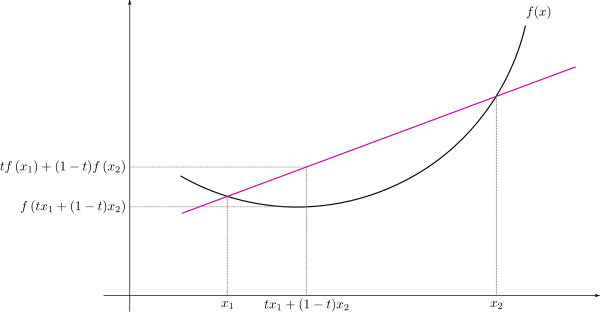
\includegraphics[width=0.7\textwidth]{convex.png}
\caption{凸函数的割线在该函数图像的上方}
\end{figure}

一般形式:
对于任意点集$\{x_i\}$,若$\lambda_i\ge 0$且$\sum_i\lambda_i=1$,使用数学归纳法,可以证明凸函数f(x)满足:
\begin{equation}
f(\sum_i\lambda_ix_i)\le \sum_i\lambda_i f(x_i) \label{eq:jensen}
\end{equation}

该式被称为Jensen不等式。

在概率论中,如果X是一个随机变量,$\varphi$是一个凸函数:
\begin{equation}
\varphi(\mathrm{E}[X])\le \mathrm{E}[\varphi(X)]
\end{equation}

\subsection{证明}

\begin{proof}
\begin{enumerate}
\item n=1,2时,由凸函数的定义成立。
\item 假设$n=k$时,公式\eqref{eq:jensen}成立。
\item n=k+1时
\begin{align}
f(\sum_{i=1}^{k+1}\lambda_i x_i) 
&=f(\lambda_{k+1}x_{k+1}+\sum_{i=1}^k\lambda_i x_i) \\
&=f(\lambda_{k+1}x_{k+1}+(1-\lambda_{k+1})\sum_{i=1}^k\eta_i x_i) \label{eq:m+1}
\end{align}
其中
\begin{equation}
\eta_i=\frac{\lambda_i}{1-\lambda_{k+1}} 
\end{equation}
由公式\eqref{eq:twopoint}的结论和公式\eqref{eq:m+1}有:
\begin{equation}
f(\sum_{i=1}^{k+1}\lambda_i x_i)\le \lambda_{k+1}f(x_{k+1})+(1-\lambda_{k+1})f(\sum_{i=1}^k\eta_i x_i)) \label{eq:mmm}
\end{equation}

注意到$\lambda_i$满足:
\begin{equation}
\sum_{i=1}^{k+1}\lambda_i=1
\end{equation}

因此:
\begin{equation}
\sum_{i=1}^k\lambda_i=1-\lambda_{k+1}
\end{equation}
因此$\eta_i$也满足:
\begin{equation}
\sum_{i}^k\eta_i=\frac{\sum_{i=1}^k\lambda_i}{1-\lambda_{k+1}}=1 \label{eq:eta}
\end{equation}
由公式\eqref{eq:jensen}和\eqref{eq:eta}得到:
\begin{equation}
\sum_{i=1}^kf(\eta_ix_i) \le \sum_{i=1}^{k}\eta_if(x_i) \label{eq:eta2}
\end{equation}
由公式\eqref{eq:mmm}和式\eqref{eq:eta2}:
\begin{equation}
f(\sum_{i=1}^{k+1}\lambda_ix_i)\le \lambda_{k+1}f(x_{k+1})+(1-\lambda_{k+1})\sum_{i=1}^k\eta_if(x_i)=\sum_{i=1}^{k+1}\lambda_if(x_i)
\end{equation}

因此$i=k+1$时,Jensen不等式成立。
\end{enumerate}
综上,Jensen不等式成立。
\end{proof}

\section{柯西不等式}

柯西不等式(Cauchy-Schwarz inequality)是数学中最重要的不等式之一,对于内积空间中的任意两个向量$\mathbf u,\mathbf v$有:
\begin{equation}
|\langle \mathbf u,\mathbf v\rangle|^2\le \langle \mathbf u,\mathbf u\rangle \cdot\langle \mathbf v,\mathbf v\rangle
\end{equation}
其中$\langle\cdot,\cdot\rangle$是内积。在欧几里得空间中,即:
\begin{equation}
\left(\sum _{i=1}^{n}u_{i}v_{i}\right)^{2}\leq \left(\sum _{i=1}^{n}u_{i}^{2}\right)\left(\sum _{i=1}^{n}v_{i}^{2}\right)
\end{equation}


引入向量的范数,则该不等式可以写作:
\begin{equation}
|\langle\mathbf u,\mathbf v\rangle|\le \|\mathbf u\|\cdot\|\mathbf v\|
\end{equation}
当前仅当$\mathbf u$和$\mathbf v$线性相关时取等号。

\subsection{证明}

\begin{proof}
下面分两种情况讨论。

\begin{enumerate}[1$^\circ$]
\item 平凡情形:$\mathbf v=0$,该定理显然成立。
\item 假定$\mathbf v\neq 0$ 令$\lambda=\langle u,v\rangle/\|v\|^2$
\begin{align}
0 &\le \|u-\lambda\cdot v\|^2 \\
&=\langle u,u\rangle-\langle\lambda\cdot v,u\rangle-\langle u,\lambda\cdot v\rangle+\langle\lambda\cdot v,\lambda\cdot v\rangle \\
&=\langle u,u\rangle-\lambda\langle v,u\rangle-\lambda\langle u,v \rangle+\lambda^2\langle v,v\rangle \\
&=\|u\|^2-2\lambda\langle u,v\rangle+\lambda^2\|v\|^2 \\
&=\|u\|^2-2\frac{|<u,v>|^2}{\|v\|^2}+\frac{|\langle u,v\rangle|^2}{\|v\|^2} \\
&=\|u\|^2-\frac{|\langle u,v\rangle|^2}{\|v\|^2}
\end{align}
因此:$|\langle u,v\rangle |\le \|u\|\cdot\|v\|$成立。
\end{enumerate}
\end{proof}

\subsection{推广}
\paragraph{积分形式}
对于平方可积的复值函数,有:
$$
\left|\int f(x)\bar{g(x)}\ud x\right|^2\le \int |f(x)|^2\ud x\cdot\int |g(x)|^2\ud x
$$

\paragraph{期望形式}
设X,Y为任意两个随机变量,有:
\begin{equation}
[\mathbf E(XY)]^2\le \mathbf E(X^2)\mathbf E(Y^2)
\end{equation}

以下证明:
\begin{equation}
g(t)= \mathbf E((tX-Y)^2)=t^2(\mathbf E(X^2))-2t\mathbf E(XY)+\mathbf E(Y^2)
\end{equation}
\begin{equation}
\because (tX-Y)^2\ge 0,g(t)\ge 0
\end{equation}
\begin{equation}
\Delta=(2\mathbf E(XY))^2-4(\mathbf E(X^2)\mathbf E(Y^2))\le 0
\end{equation}

当且仅当$tX=Y$时有$g(t)=0$
所以:
\begin{equation}
[\mathbf E(XY)]^2\le \mathbf E(X^2)\mathbf E(Y^2)
\end{equation}

\subsection{拉格朗日恒等式}
在三维欧氏空间中有下列关系:

\begin{equation}
\|{\mathbf  a}\|^{2}\cdot \|{\mathbf  b}\|^{2}=({\mathbf  {a\cdot b}})^{2}+|\mathbf a\times\mathbf  b|^2
\end{equation}

\section{赫尔德不等式}


\section{排序不等式}

排序不等式又称排序原理,设$a_1\le a_2\le \cdots a_n,b_1\le b_2\le\cdots b_n$,$c_1,c_2,\cdots,c_n$是$b_1,b_2,\cdots,b_n$的任一排列,则
\begin{equation}
 \underbrace{a_1b_n+a_2b_{n-1}+\cdots+a_nb_1}_{\text{反序和}}\le \underbrace{a_1c_1+a_2c_2+\cdots a_nc_n}_{\text{乱序和}}\le\underbrace{a_1b_1+a_2b_2+\cdots+a_nb_n}_{\text{顺序和}} 
\end{equation}

当且仅当$a_1=a_2=\cdots=a_n$或$b_1=b_2=\cdots b_n$时,反序和等于顺序和。

\subsection{证明}
设$a_1\le a_2\le \cdots a_n$,$b_1\le b_2\le \cdots b_n$为两组实数,$c_1,c_2,\cdots c_n$是$b_1,b_2,\cdots,b_n$的任一排列,因为$b_1,b_2,\cdots,b_n$的全排列只有$n!$个,所以:
\begin{equation}
S=a_1c_1+a_2c_2+\cdots+a_nc_n \label{eq:ac}
\end{equation}

的不同的值也只有有限个(个数$\le n!$),其中必有最大值和最小值。

考虑式\eqref{eq:ac},若$c_1\neq b_1$,则有某$c_k=b_1(k>1)$,$c_1>c_k$,将\eqref{eq:ac}对换,得
\begin{equation}
S'=a_1c_k+\cdots +a_kc_1+\cdots a_nc_n \label{eq:ak}
\end{equation}

\eqref{eq:ak}-\eqref{eq:ac}得:
\begin{equation}
S'-S=a_1c_k+a_kc_1-a_1c_1-a_kc_k=(a_k-a_1)(c_1-c_k)\ge 0
\end{equation}

这说明将\eqref{eq:ak}调换为$a_1b_1$后,和式不减小。

若$c_1=b_1$,则转而考察$c_2$,并进行类似讨论。

类似地,可以证明,将\eqref{eq:ac}中的第一项换为$a_1b_1$,第二项换位$a_2b_2$后,和式不减小。

如此下去,经过有限步调整,可以一切和数中,最大和数所对应的情况只能是数组$\{c_i\}$由小到大排序的情况,最大和数是顺序和。

同理可证,最小和数是反序和。


\section{切比雪夫总和不等式}

\section{三角不等式}

\section{闵可夫斯基不等式}


% \backmatter
\begin{thebibliography}{99}
\bibitem{wiki}Wikipedia
\bibitem{ineq}不等式的解题方法与技巧。
\bibitem{ineqb}贝努利不等式的几个推论及应用。
\end{thebibliography}


\end{document}